\chapter{Caracterización Magnética}

Para la caracterización magnética se determinaron curvas de magnetización en
función de la temperatura a diferentes campos magnéticos (100 Oe a 25 kOe) y
magnetización en función del campo magnético (entre -30 kOe a 30 kOe) a
diferentes temperaturas, para el sistema
\ce{Lu3Al_{5-X}Fe_{x}O12}:\ce{Ce^{3+}}.\\

En la Figura \ref{fig:suce} se muestran las curvas para los compuestos con $x\leq 1.5$
en las
cuales se aplicaron los procedimientos ZFC (enfriando en ausencia de campo
magnético, aplicando el campo a bajas temperaturas y midiendo mientras la
temperatura aumenta) y FC (midiendo mientras se enfría en presencia de campos
magnéticos) bajo la aplicación de un campo H = 1 kOe. El comportamiento
observado evidencia una característica típicamente paramagnética, con un
decrecimiento abrupto a bajas temperaturas y asintótico a altas temperaturas.\\

Se percibe una pequeña diferencia entre las curvas ZFC-FC, este
comportamiento puede estar asociado a efectos de anisotropía de forma debido al
carácter granular de los materiales, ya que no todos tienen la misma forma con
lo cual puede afectarse el acoplamiento magnético entre ellos, haciendo que los
espines magnéticos respondan de manera diferente a la aplicación del campo
entre los diferentes granos de diversos tamaños y formas presentes, resultando
en un pequeño aumento de la susceptibilidad, pero también en un efecto de
desorden que genera irreversibilidad entre los dos procedimientos de medida
(ZFC-FC) \cite{bustos2018analisis}. La curva de susceptibilidad para los cuatro sistemas son
esencialmente la misma, salvo por una pequeña bifurcación observable para un
valor de temperatura de 71.77 K para el compuesto con x = 0. Lo cual es
atribuido a efectos de anisotropía de forma relacionada con el carácter
granular del material conforme se evidenció en el análisis presentado en el capítulo
\ref{MEB}.\\

Las curvas obtenidas a 1 kOe se ajustaron a la fórmula de Curie-Weiss en el
rango de temperatura de (150$-$400) K. El rango de ajuste dependió de la muestra
debido al efecto de campo cristalino.\\

\begin{equation}
  \frac{1}{\chi} = \frac{1}{\chi_0+\frac{C}{T-\theta_{CW}}}
  \label{eqn:suce}
\end{equation}

Empleando la Ecuación \ref{eqn:suce}, se obtuvo la constante de Curie C, la
temperatura de
Curie-Weiss $\theta_{CW}$ y la susceptibilidad paramagnética independiente de
la
temperatura $\chi_0$ (ver Tabla \ref{tab:suce}) \cite{gaona2021possible}. El valor de la constante C se
utilizó para
calcular el momento magnético efectivo de los compuestos. La muestra x = 0.5
muestra una mayor contribución paramagnética, lo que sugiere una heterogeneidad
local \cite{talik2017properties}.\\

%%Tabla
\begin{table}[h]
  \centering
  \caption{Parámetros obtenidos después del ajuste del inverso de la susceptibilidad}
  \label{tab:suce}
  \begin{tabular}{
      >{\columncolor[HTML]{FFFFFF}}l
      >{\columncolor[HTML]{FFFFFF}}l
      >{\columncolor[HTML]{FFFFFF}}l
      >{\columncolor[HTML]{FFFFFF}}l
      >{\columncolor[HTML]{FFFFFF}}l
      >{\columncolor[HTML]{FFFFFF}}l
      >{\columncolor[HTML]{FFFFFF}}l}
    \hline
    \cellcolor[HTML]{FFFFFF}                                                                                                              &
    \cellcolor[HTML]{FFFFFF}                                                                                                              &
    \cellcolor[HTML]{FFFFFF}                                                                                                              &
    \cellcolor[HTML]{FFFFFF}                                                                                                              &
    \cellcolor[HTML]{FFFFFF}                                                                                                              &
    \multicolumn{2}{l}{\cellcolor[HTML]{FFFFFF}$\mu_{eff}^{cal} (\mu_B)$}                                                                   \\ \cline{6-7}
    \multirow{-2}{*}{\cellcolor[HTML]{FFFFFF}Muestra}                                                                                     &
    \multirow{-2}{*}{\cellcolor[HTML]{FFFFFF}\begin{tabular}[c]{@{}l@{}}$\chi_0$\\ $emu\cdot mol^{-1}$\end{tabular}} &
    \multirow{-2}{*}{\cellcolor[HTML]{FFFFFF}\begin{tabular}[c]{@{}l@{}}$\theta_{CW}$\\ (K)\end{tabular}}                       &
    \multirow{-2}{*}{\cellcolor[HTML]{FFFFFF}\begin{tabular}[c]{@{}l@{}}C\\ $emuK \cdot mol^{-1}$\end{tabular}}      &
    \multirow{-2}{*}{\cellcolor[HTML]{FFFFFF}\begin{tabular}[c]{@{}l@{}}$\mu_{eff}^{exp}$\\ $\mu_B$\end{tabular}}                   &
    \ce{Fe^{2+}}                                                                                                                          &
    \ce{Fe^{3+}}                                                                                                                            \\ \hline
    x = 0                                                                                                                                 &
    $1.802x10^{-4}$                                                                                                                       &
    --                                                                                                                                    &
    --                                                                                                                                    &
    --                                                                                                                                    &
    0.0                                                                                                                                   &
    0.0                                                                                                                                     \\
    x = 0.5                                                                                                                               &
    $5.184x10^{-4}$                                                                                                                       &
    -2.82                                                                                                                                 &
    1.00                                                                                                                                  &
    2.81                                                                                                                                  &
    4.74                                                                                                                                  &
    4.19                                                                                                                                    \\
    x = 1.0                                                                                                                               &
    $0.179x10^{-4}$                                                                                                                       &
    -9.29                                                                                                                                 &
    1.65                                                                                                                                  &
    3.62                                                                                                                                  &
    6.71                                                                                                                                  &
    5.92                                                                                                                                    \\
    x = 1.5                                                                                                                               &
    $1.550x10^{-3}$                                                                                                                       &
    -2.58                                                                                                                                 &
    2.65                                                                                                                                  &
    4.59                                                                                                                                  &
    8.22                                                                                                                                  &
    7.25                                                                                                                                    \\ \hline
  \end{tabular}
\end{table}


%%Figura

\begin{figure}[H]
  \centering%

  \includegraphics[width=14cm]{Kap6/FIG1.jpg}%
  \caption{Comportamiento de la susceptibilidad en función de la temperatura
  bajo la aplicación de un campo magnético H = 1 kOe para los compuestos
  \ce{Lu3Al_{5-x}Fe_{x}O_{12}}:\ce{Ce^{3+}} con $x \leq 1.5$. Recuadro: Inverso
  de la susceptibilidad en función de la temperatura para el sistema con x = 1.0.
  }
  \label{fig:suce}
\end{figure}

Es evidente que la extrapolación de la recta del inverso de la susceptibilidad
no corta con el eje de la temperatura en el origen, por lo cual se establece
que los materiales no presentan totalmente una respuesta paramagnética, como lo
muestra el recuadro de la Figura \ref{fig:suce} para el compuesto con x = 1.0. Este
tipo de
comportamiento es típico de materiales antiferromagnéticos, lo cual puede
confirmarse con el valor negativo de $\theta_{CW}$. Además de que los iones
\ce{Fe^{+3}}, en los
dos sitios diferentes (a) y (d), están fuertemente acoplados
antiferromagnéticamente por sus propias interacciones mutuas \cite{guillot1977magnetic}.\\

El momento efectivo experimental se determinó con la fórmula
$\mu_{eff}^{exp}=2.82(C)^{1/2}$ y el valor teórico del momento efectivo,
($\mu_{eff}^{cal}$), se calculó de acuerdo con la ecuación \ref{eqn:momento}.

\begin{equation}
  \mu_{eff}^{cal}=\sqrt{x\cdot (\mu_{eff}^{teo} \ce{Fe^{3+/2+}})^2}
  \label{eqn:momento}
\end{equation}

Los resultados obtenidos de los momentos efectivos según la Tabla \ref{tab:suce}, son
menores que los esperados de la contribución del momento magnético de solo
espín para el hierro (\ce{Fe^{2+}} = 6.71 $\mu_{B}$ y \ce{Fe^{3+}} = 5.92
$\mu_B$). Esto se puede atribuir
al método de síntesis y a factores que promueven cambios en el orden magnético
de los movimientos catiónicos debido a distorsiones estructurales que modifican
el momento magnético neto \cite{banos2018enhancement}. Como vacantes de oxígeno que dan como
resultado
la creación de un estado de valencia mixto para el hierro \ce{Fe^{2+}/Fe^{3+}},
resaltando que el ion \ce{Fe^{2+}} evidencia un momento magnético más bajo en
comparación con \ce{Fe^{3+}}, por lo que su presencia da como resultado una
disminución
del momento magnético en los compuestos \cite{hussain2019growth}.\\

La Figura \ref{fig:zfc} muestra las curvas de magnetización en función de la
temperatura a
diferentes campos magnéticos (100 Oe a 25 kOe) para los sistemas con $x \geq
  2.0$,
donde se emplearon los procesos ZFC-FC. A modo general las curvas
termomagnéticas demostraron una disminución no lineal de la magnetización con
el aumento de la temperatura y una disminución de la magnetización a menor
campo magnético, esto es atribuido a que el orden de los momentos magnéticos de
los átomos se encuentra en un estado aleatorio \cite{ramesh20173}. Al observar los
recuadros de la Figura \ref{fig:zfc}
es evidente que para un campo de H = 100 Oe los compuestos presentaron un
comportamiento
diferente en comparación con valores mayores de H.\\

\begin{figure}[H]
  \centering%

  \includegraphics[width=\textwidth]{Kap6/FIG2.jpg}%
  \caption{Curvas de magnetización ZFC-FC a diferentes campos magnéticos (100
  Oe a 25 kOe) del sistema \ce{Lu3Al_{5-x}Fe_{x}O_{12}}:\ce{Ce^{3+}} con $x \geq
    2.0$. Recuadros: Ampliación de las curvas con un campo de H = 100 Oe. (a) x =
  2.0, (b) x = 2.5, (c) x = 3.0, (d) x = 3.5, (e) x = 4.0 y (f) x = 4.5. }
  \label{fig:zfc}
\end{figure}

El comportamiento presentado a H = 100 Oe es concordante con nanopartículas
\@\ce{Fe3O4}
\cite{singh2017shape,gaona2021characterization}. De esta manera, para el proceso ZFC la muestra se enfría a baja
temperatura ($\sim $ 50 K), donde el momento magnético neto es insignificante,
ya que
el momento magnético de cada partícula individual está orientado al azar.
Cuando se aplica el campo magnético externo, los momentos orientados
aleatoriamente comienzan a alinearse en la dirección del campo. Por lo tanto,
el momento magnético neto aumenta gradualmente y alcanza el máximo marcado como
$T_{irr}$ (229.58, 111.77, 274.78, 304.35 y 364.75 K para x = 2.0, 3.0, 3.5,
4.0 y
4.5, respectivamente).\\

La temperatura a la que la magnetización es máxima se conoce como temperatura
de bloqueo ($T_B$), la cual se define como la temperatura a la que la energía
térmica está en equilibrio con la energía de los momentos magnéticos alineados
\cite{shao2018preparation}.
A medida que la temperatura aumenta más que la temperatura de bloqueo, la
energía térmica comienza a destruir la alineación de los momentos y, por lo
tanto, resulta en una disminución de la magnetización por encima de $T_B$
(197.5,
67.7, 164.5, 172.2 y 159.2 K, para x = 2.0, 3.0, 3.5, 4.0 y 4.5
respectivamente).
Además, cabe señalar a partir de los gráficos, las curvas FC
y ZFC se comportan de manera similar por encima de la temperatura de bloqueo,
que es diferente para todas las muestras.\\

La Figura \ref{fig:magneti} muestra los resultados de magnetización en función del campo
magnético a temperatura ambiente (T = 300K) de todos los compuestos. Se observó
que las propiedades magnéticas de las muestras cambiaban al aumentar x. Los
resultados obtenidos para los sistemas con x = 0.5, 1.0 y 1.5 (Ver Figura
\ref{fig:magneti}a)
evidenciaron un comportamiento paramagnético con una coercitividad nula para x=
0.5
y una alta coercitividad para x = 1.0 y 1.5 con valores de Hc 632.5 y
505.1 Oe respectivamente \cite{musa2017structural}. Por otro lado, para los compuestos con x =
2.0,
2.5 y 3.0, muestran un comportamiento ferromagnético que es más pronunciado a
mayor contenido de Al. Para los sistemas con x = 3.5, 4.0 y 4.5, las curvas
obtenidas son típicas de materiales ferrimagnéticos, atribuido a la interacción
de superintercambio dominante entre los sitios (a) y (d) del \ce{Fe} que hacen
que
sus momentos magnéticos sean antiparalelos \cite{yamagishi2005ferrimagnetic}. Los resultados de los
parámetros magnéticos son influenciados por el tamaño de partícula de los
sistemas
\cite{tan2008room}. Fue evidente que a mayor tamaño de partícula mayor fue el valor de Ms
(1.02, 3.90 y 10.38 emu/g para 3.5, 4.0 y 4.5 respectivamente), además de que
los valores obtenidos son menores a los reportados.\\

\begin{figure}[h]
  \centering%

  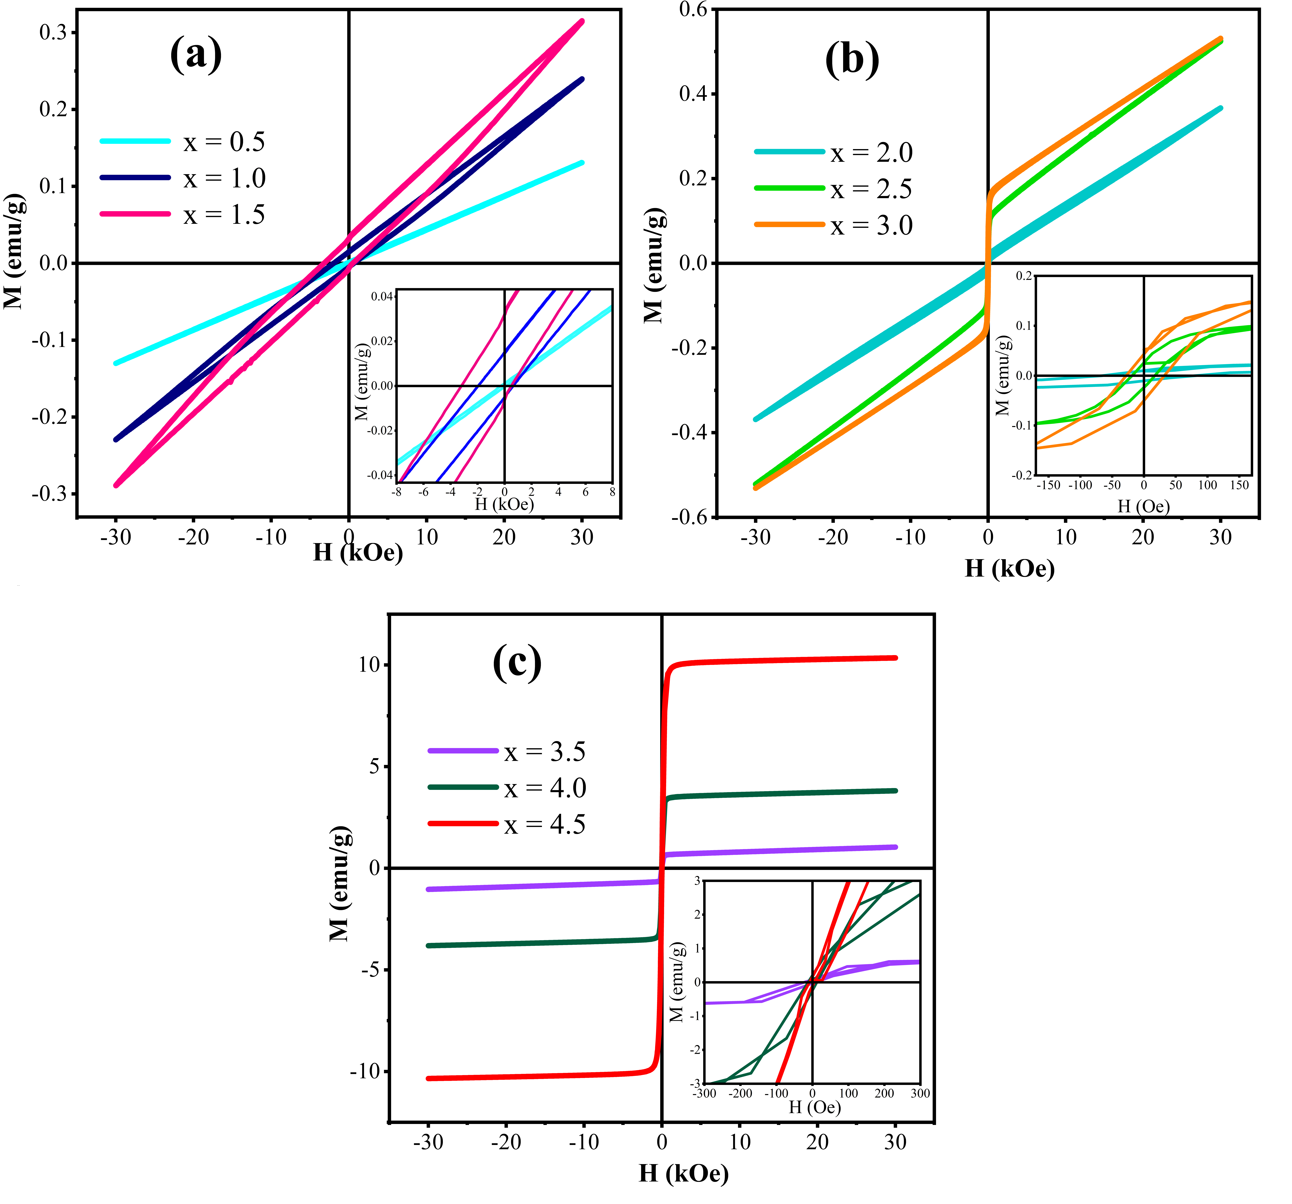
\includegraphics[width=\textwidth]{Kap6/MH.png}%
  \caption{Curvas de magnetización en función del campo magnético a
  temperatura
  ambiente del sistema \ce{Lu3Al_{5-x}Fe_{x}O_{12}}:\ce{Ce^{3+}}  con (a) $x \leq 1.5$, (b) $x \leq 3.0$ y (c)  $x \leq 4.5$. }\label{fig:magneti}
\end{figure}

Los resultados muestran que la concentración de Al afecta la magnetización de
saturación, $M_s$, y coercitividad, $H_c$, de las muestras. Los valores de
$M_s$
aumentan a medida que aumenta la concentración de Al. Por tanto, la reducción
de Ms en relación con lo reportado es el resultado de que los iones de Al
paramagnéticos sustituyen a los iones de Fe ferromagnéticos, lo que disminuye
el momento magnético neto resultante de la interacción de superintercambio
entre los sitios (a) y (d) del granate. El valor creciente de la coercitividad
a mayor contenido de x se debe a la forma y anisotropía magnetocristalina de
granos grandes. Para un tamaño de grano más grande la anisotropía desaparecerá,
pero la anisotropía magnetocristalina permanecerá \cite{hapishah2017phase} (ver Figura
\ref{fig:mr}).\\

\begin{figure}[t]
  \centering%

  \includegraphics[width=11cm]{Kap6/FIG4.jpg}%
  \caption{Magnetización de saturación en función de la concentración para muestras de granate \ce{Lu3Al_{5-x}Fe_{x}O_{12}}:\ce{Ce^{3+}} con $x \geq 2.0$.}
  \label{fig:mr}
\end{figure}
